\documentclass[tikz,border=8pt]{standalone}
% Shared look for every TikZ diagram. Load with \input{../../tools/tikz-style.tex}
\usepackage[T1]{fontenc}
\usepackage{lmodern}
\renewcommand{\sfdefault}{lmr}  % diagrams use the same serif as the text
\usetikzlibrary{arrows.meta, positioning, shapes.geometric, calc, fit, backgrounds}
\definecolor{cblue}{HTML}{4C78A8}
\definecolor{corange}{HTML}{F58518}
\definecolor{cgreen}{HTML}{54A24B}
\definecolor{cred}{HTML}{E45756}
\definecolor{cpurple}{HTML}{B279A2}
\definecolor{cgrey}{HTML}{6B6B6B}
\tikzset{
  every picture/.style={font=\sffamily, line width=1.2pt},
  box/.style={draw=#1, fill=#1!12, rounded corners=4pt, align=center, inner sep=7pt, minimum height=1.1cm},
  box/.default=cgrey,
  arrow/.style={-{Stealth[length=3mm]}, draw=cgrey, line width=1.4pt},
  title/.style={font=\sffamily\bfseries\Large},
  note/.style={font=\sffamily\small, text=cgrey, align=center},
}
\AtBeginDocument{\hyphenpenalty=10000 \exhyphenpenalty=10000}

\begin{document}
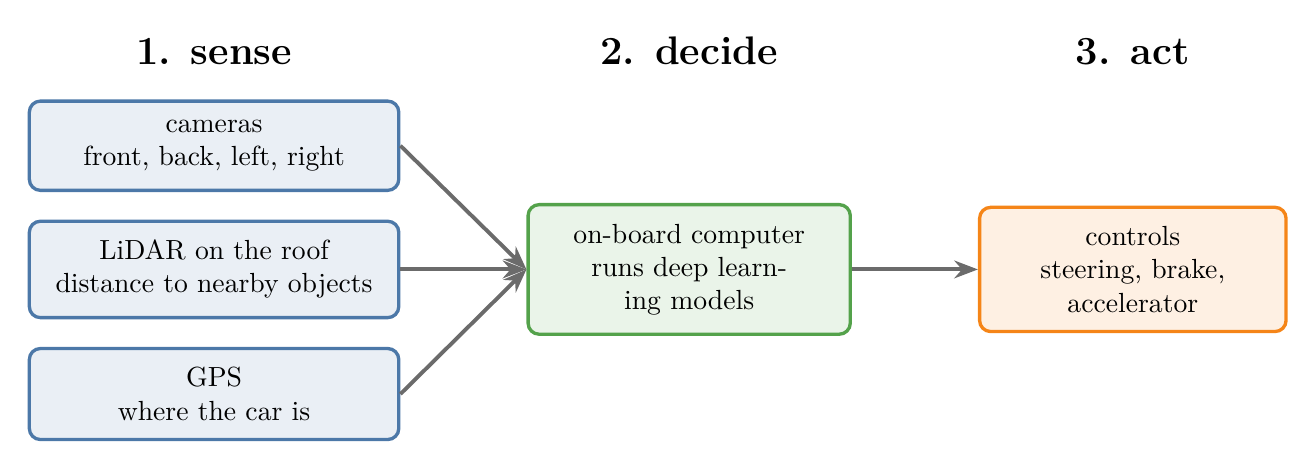
\begin{tikzpicture}[node distance=0.35cm and 1.6cm]
  \node[box=cblue, text width=4.2cm] (cam) {cameras\\front, back, left, right};
  \node[box=cblue, text width=4.2cm, below=of cam] (lidar) {LiDAR on the roof\\distance to nearby objects};
  \node[box=cblue, text width=4.2cm, below=of lidar] (gps) {GPS\\where the car is};
  \node[box=cgreen, text width=3.6cm, right=of lidar] (pc) {on-board computer\\runs deep learning models};
  \node[box=corange, text width=3.4cm, right=of pc] (ctl) {controls\\steering, brake, accelerator};
  \foreach \s in {cam, lidar, gps} \draw[arrow] (\s.east) -- (pc.west);
  \draw[arrow] (pc) -- (ctl);
  \node[title, above=0.3cm of cam] {1. sense};
  \node[title] at (pc |- cam.north) [above=0.3cm] {2. decide};
  \node[title] at (ctl |- cam.north) [above=0.3cm] {3. act};
\end{tikzpicture}
\end{document}
